\documentclass[11pt,a4paper]{article}
\usepackage[utf8]{inputenc}
\usepackage[english]{babel}
\usepackage[T1]{fontenc}
\usepackage{amsmath}
\usepackage{amsfonts}
\usepackage{amssymb}
\usepackage{graphicx}
\usepackage{array}
\usepackage{multirow}
\usepackage[left=2cm,right=2cm,top=2cm,bottom=2cm]{geometry}
\author{Guillem Tocabens}
\title{First measurements}
\begin{document}

\begin{titlepage}

\newcommand{\HRule}{\rule{\linewidth}{0.5mm}} % Defines a new command for the horizontal lines, change thickness here

\center % Center everything on the page
 
%----------------------------------------------------------------------------------------
%	HEADING SECTIONS
%----------------------------------------------------------------------------------------

\textsc{\LARGE Lund University}\\[1.5cm] % Name of your university/college
\textsc{\Large Report from internship in the nuclear division}\\[0.5cm] % Major heading such as course name
\textsc{\large }\\[0.5cm] % Minor heading such as course title

%----------------------------------------------------------------------------------------
%	TITLE SECTION
%----------------------------------------------------------------------------------------

\HRule \\[0.4cm]
{ \huge \bfseries Characterisation of a square type HPGe crystal and development of the Lund germanium detector scanning system}\\[0.4cm] % Title of your document
\HRule \\[1.5cm]
 
%----------------------------------------------------------------------------------------
%	AUTHOR SECTION
%----------------------------------------------------------------------------------------

\begin{minipage}{0.4\textwidth}
\begin{flushleft} \large
\emph{Author:}\\
Guillem \textsc{Tocabens}\\ % Your name
\end{flushleft}
\end{minipage}
~
\begin{minipage}{0.4\textwidth}
\begin{flushright} \large
\emph{Supervisors:} \\
Luis \textsc{Sarmiento} \\
Dirk \textsc{Rudolph} % Supervisor's Name
\end{flushright}
\end{minipage}\\[2cm]

% If you don't want a supervisor, uncomment the two lines below and remove the section above
%\Large \emph{Author:}\\
%John \textsc{Smith}\\[3cm] % Your name

%----------------------------------------------------------------------------------------
%	DATE SECTION
%----------------------------------------------------------------------------------------

{\large \today}\\[2cm] % Date, change the \today to a set date if you want to be precise

%----------------------------------------------------------------------------------------
%	LOGO SECTION
%----------------------------------------------------------------------------------------

\begin{figure}[!h]
\centering

\includegraphics[scale=0.6]{Logo.png}
\end{figure} % Include a department/university logo - this will require the graphicx package
 
%----------------------------------------------------------------------------------------

\vfill % Fill the rest of the page with whitespace



\end{titlepage}


\newpage
\tableofcontents
\thispagestyle{empty}
\newpage

\section{Introduction}

Nuclear structure continues to be an active branch in the field of nuclear physics, because there is still a lot to discover. One of the things that is recognized among the nuclear physics' researchers is the existence of magic numbers. Nuclei counting a magic number of protons, neutrons or both are usually more stable than neighbouring nuclei, at least if nuclei not far away from the line of stability are considered (see Figure~\ref{Nuclchart}). Today, those numbers are known up to a certain point. Indeed, nuclei with $N, Z = 2, 8, 20, 28, 50, 82$ and $N = 126$ are more stable than others. Nevertheless, as soon as heavier nuclei (in the sense of nuclei with more protons and/or neutrons) are considered, no magic number of protons or neutrons have been experimentaly observed. Theoretically some models are being developed and predict, for example, that $N = 184$ and $Z = 114$ could be the next magic numbers for neutrons and protons, respectively. The search for an "island of stability" in the region of superheavy elements, counting more than 103 protons, is thus very important to get the chance to observe stable (regarding spontaneous fission) superheavy elements.

This process of researching the island of stability is not straight forward at all and requires at least two different steps. First of all, these superheavy elements need to be created. One widely used technique is via fusion-evaporation reactions~: a beam of stable isotopes is accelerated towards a target made of a different element. The elements can fuse if the energy is larger than the Coulomb barrier. The product evaporates neutrons, protons or other light particles, such as $\alpha$ particles. This way, heavy and superheavy elements can be created, like in an experiment conducted in 2012 at the Helmholtz Centre for Heavy Ion Research (GSI, in Germany). A beam of $^{48}$Ca was accelerated towards a target of $^{243}$Am to create an element containing 115 protons recently named moscovium, Mc \cite{element115}.
The process of creation of superheavy elements is tedious since the cross sections for fusion-evaporation reactions are ridiculously little. In former experiments, only a few elements where observed.

The second step in the search for the island of stability actually contains two different processes which are closely linked~: observation through decay and identification of the created element. Even though the elements which are looked for are stable regarding spontaneous fission, they still decay rather quickly through $\alpha$ decay. Half-lives, $T_{1/2}$, of known element 115 isotopes are on the order of hundred(s) of milliseconds, for instance. The emitted $\alpha$ particles can thus be detected and their energy can be extracted to reconstruct the $\alpha$-decay chain of the isotope. But as the knowledge about superheavy elements is far from complete, it is hard to place that chain on the nuclidic chart and thus determine what element was created in the first place. Nonetheless, after emitting an alpha particle, superheavy elements can end in an excited state of the daughter. Rearrangements can then happen and the element may decay to its ground state through electron capture, which emits X-rays of about $150~keV$ (decay into the atomic K shell) or $30~keV$ (decay into the atomic L shell) for example. X-ray energies are specific to each element. Therefore, if they are detected a short time (some nanoseconds or less) after the alpha particle was detected, the term used is "in prompt coincidence", it is possible to recognize the corresponding element. If this happens, the alpha decay chain can then be identified and, consequently, the created element too.

\begin{figure}[!h]
\centering
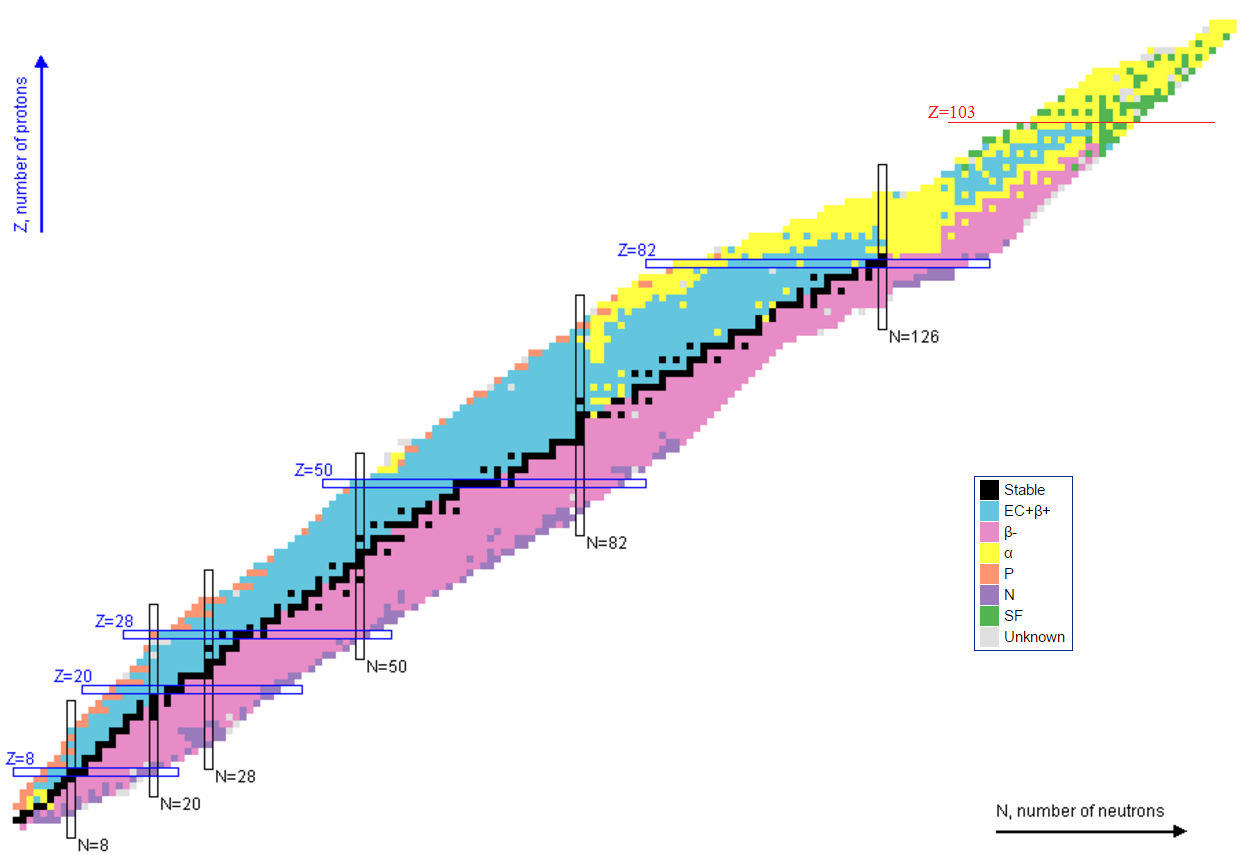
\includegraphics[scale=0.6]{Nuclchart2.png}
\caption{Chart of nuclides, classifying the nuclides with respect to their number of protons and neutrons. The know magic numbers are given on the chart as long as the nuclei having a magic number of protons, in blue, or of neutrons, in black. On that chart the colors represent the modes of decay of each nuclide, emphasized by the small squares. The region of interest is the one of the superheavy elements, up from the red line on the chart.}
\label{Nuclchart}
\end{figure}

In the past decades, new superheavy elements were discovered, up to element $Z = 118$, Oganesson Og, first synthesized in 2002 and confirmed in 2015 \cite{element118}.
In the perspective of finding the next superheavy element, $Z = 119$, new detectors must be developped with, for example, a high resolution in the X-ray domain. This thesis concentrates on the characterization of such a new system which should have a high resolution in both $\gamma$-ray domain (up to some MeV) and X-ray domain. Indeed, this detector will also be used to study known superheavy elements and determine their structure and decay.

The studied detector is a semi-conductor detector using a high-purity germanium crystal with coaxial geometry. The main difference with usual germanium detectors is that while coaxial detectors are cylindrical, the new detector will have a cubic geometry. Informatic simulations were performed to determine the right geometry to use for that crystal but also to determine how to pack four crystals into a "clover" of four detectors. However, the main topic of this thesis is to be able to characterize the new detector by means of a scanning system. This system would be used to study the response of the crystal to a collimated beam at a given number of points of its surface The whole functioning of the system will be developed in this thesis.

But before being able to scan the crystal, the main part of the project was to build a setup that could match the needs of the experiments that would be performed with the detector. The goal here was to develop everything, starting by drawing the setup as it should look like in the end, purchasing all the needed material and pieces, and finally building the whole setup once the pieces were available. Section \ref{scansystem} will thus be dedicated to explain the development of such a system and the different steps of the process while Section \ref{analysis} will present measurements performed with two different prototypes of detectors. Some needed physical background is introduced in Section \ref{theory} but it is assumed that a basic knowledge on semi-conductor detectors is already in the hands of the reader.

\newpage

\section{Theory and background} \label{theory}

\subsection{The crystal}

The studied crystal has the same caracteristics as coaxial crystals, the only difference being its squared geometry while coaxial crystals have circular geometry. The crystal is a closed-end coaxial crystal, meaning its geometry is squared with a hole in it that does not go all the way in the volume (see Figure~\ref{geo}). The crystal is oriented such that the incoming photons hit the part without the hole first. As a germanium detector uses a depletion zone to detect photons (\cite{phot}), it must contain a p- and n-dopped faces. The p-contact is made by adding an electron donor, here Boron is implanted on the outer surface of the Germanium crystal, and the n-contact is made by adding a hole donor, Lithium, on the inner surface (the surface of the hole) of the crystal. Both these added layers function as dead layers\footnote{A dead layer is a volume that does not contribute to the detection of photons while it is not in the depletion zone, due to its too high level of impurities.} and are quite important on the n-side since the layer is measured to be $0.5~mm$ to $1~mm$ thick.

In order to protect the crystal from oxidation, a passivation layer is added on the inner surface of the crystal. This layer is made with SiO$^2$, which is not optimal for germanium crystal as both crystal lattices does not fit. This could imply perturbations in the electric field, increasing noise in the measurements. To prevent from this potential noise, a methanol passivation should be preferrable on germanium. However, such a passivation layer can't be achieved in atmosphere, but could be done in the encapsulation.

The crystal is placed in a cryostat that ensures its temperature to be as low as possible thanks to liquid nitrogen as germanium detectors need to be cooled down to work properly (\cite{Knoll}). The cooling is performed thanks to a dewar filled with liquid nitrogen that is connected to the crystal through a cooling finger. Close to the cryostat is a preamplifier that converts the signal from current to voltage and amplifies it a first time (\cite{Tsoulfanidis}). The preamplifier is then the output of the detector which can be connected to further electronic devices.

\subsection{Spectral properties} \label{spectral}

After going through different electronic modules, the signal detected by the crystal is sent to a computer to be analyzed. The collected data presents a number of counts detected by the crystal for each channel in the multichannel analyzer\footnote{A multichannel analyzer, MCA, sorts the digital values it receives from an analog to digital converter, ADC, and stores them to be used on a computer.}. As a channel number has no physical meaning, the detector needs to be calibrated using a known source in order to associate an energy to each channel. The result is then a plot of the detected number of counts for each given energy which is called a spectrum. This spectra are of main importance as they allow to determine some of the spectral properties of the crystal.

The first property that is interesting to determine is the resolution of the detector as it gives the uncertainty on the measures done with the detector. The resolution is determined by fitting Gaussians to the peaks in the spectra and calculating their Full Width at Half Maximum, FWHM, which is directly a measure of the uncertainty on the energy and thus the resolution of the detector. Resolution varies with the energy of the detected photon and is usually better in the low-energies range than in the high-energies range. Resolution can be written as the sum of three different contributions (see \cite{Tsoulfanidis})~:

\begin{equation}
W_T = W_D^2 + W_X^2 + W_E^2
\end{equation}
where the W are the expected peak FWHM due to carrier statistics, carrier collection and electronic noise, respectively. While the contribution of electric noise is constant as a function of energy, both other contributions are energy dependent. $W_D$, the inherent statistical fluctuation in the number of created charge carriers varies with the square root of the energy of the detected photon while $W_X$, due to incomplete charge collection, varies linearly with energy (Figure~\ref{resolution}).

\begin{figure}
\centering
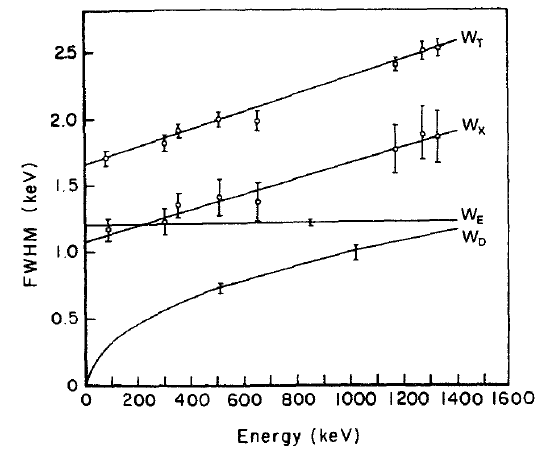
\includegraphics[scale=0.9]{resolution.png}
\caption{Plot of the different contributions to the energy resolution of a germanium detector as a function of the energy of the detected photon, from \cite{Knoll}.}
\label{resolution}
\end{figure}

Another important feature that can be determined from a spectrum is the shape of the peaks. While peaks are fitted to Gaussians, it is quite important to make sure that this approximation is true. In order to determine this, the shape factors are often used. They are estimated using the ratio between the FWHM of the peak and the Full Width at Tenth Maximum or the Full Width at Fiftieth Maximum. Considering a perfect Gaussian peak, these ratios are given by~:

\begin{equation}
\dfrac{FWTM}{FWHM} = 1.82 \text{  and  } \dfrac{FWFM}{FWHM} = 2.38
\end{equation}
They are mainly due to the electronics (too short shaping time, bad pole-zero adjustment, etc.) but can also be affected by other factors such as damages on the crystal or a too high count rate leading to pile-up.

Finally, one can be interested in calculating the peak-to-Compton ratio, which is an indicator of the performance of the detector while it gives the noise level in the detector. It is defined as being the ratio between the maximum counts of the peak at $1332.5~keV$ of a $^{60}$Co source and the average Compton height \cite{Yii}. The Compton height represents the average height of the Compton distribution, taken between $1040~keV$ and $1096~keV$ to avoid the Compton edge. The ratio is mainly influenced by the efficiency and the resolution of the detector at $1332.5~keV$. Indeed, the better the efficiency, the more counts in the peak and the same is true for resolution, thus the ratio increases with both resolution and efficiency.

\subsection{Capacitance}

As a result of the electric field present in the depletion region of a germanium detector, the crystal shows an inherent capacitance. This capacitance varies with the voltage applied to the crystal and is constant when a sufficiently high voltage is applied on the crystal. In a reversed bias regime, the capacitance decreases when the absolute value of the voltage increases thus, to make the capacitance as low as possible, the reversed bias applied to the crystal must be as high as possible. It is important to have a low capacitance in the crystal while it is one of the reasons for electric noise on the spectra. Indeed, the noise charge, which is a measure of the noise level, is proportionnal to the total capacitance in the detector. The total capacitance comes from the electronics but also in part from the crystal. Thus, it is important to minimise the capacitance in the crystal to obtain as little noise as possible and a good resolution \cite{Kephart}.

The capacitance of a semi-conductor crystal only depends on its geometry. In the case of a square crystal, the calculation had not been made but qualitatively it can be said that the capacitance is larger when the hole in the middle of the crystal is larger. The hole must then be kept as shallow as possible to get a reasonable resolution. As will be discussed further, the capacitance is not the only factor that influences resolution depending on the length of the hole and trapping can be a big issue.

\subsection{Trapping}

Trapping is an important issue when it comes to resolution in germanium detectors as it is contained in the $W_X$ term (see \ref{spectral}) corresponding to charge carrier collection. Due to the impurities and the defects in a germanium crystal, new energy states appear that can trap the electrons (or holes). When a charge carrier is trapped in such a state, there are two different possibilities~:

\begin{itemize}
\item If the trapping center can trap both types of charge carriers (electron and holes), it could happen that a second charge carrier is trapped, anihilating both and implying a loss in carriers.
\item If the trapping center can only trap one of the two types of charge carriers, the trapped carrier will stay in the trapping center for a given time and then continue its path to the collection center.
\end{itemize}
The first possibility ends up with a loss in charge carriers and thus a loss in energy resolution. For the second possibility, there are again two possible scenarios. Either the trapping time is shorter than the collection time and thus the carrier is released before the end of the collection and can still participate in the signal. In the case of a longer trapping time than the collection time, then the carrier does not participate in the signal, resulting in a loss of energy resolution and a poor shape of the peaks in the spectra \cite{Tsoulfanidis}.

Of course, the number of trapped charge carriers depends on the number of impurities in the crystal, but this is not a problem as any crystal used for detection is made to match the correct number of impurities to avoid trapping as much as possible. In the case of the studied prototype, as it has a square geometry, all the charge carriers have not the same path length to travel to the collection center in the middle of the crystal. A longer path would result in a higher probability for a charge carrier to be trapped. Thus, the length of the hole in the middle of the crystal, which is the collection center, is of primary importance to reduce the effects of trapping. With this property of trapping, a poorer resolution is also expected in the corners of the crystal compared to the middle while the path length is again increasing. This shows the importance of scanning the detector on its surface in order to improve the resolution by optimizing the analysis routine.

Finally, the amount of charges that are trapped in the trapping centers depends on the energy that is deposited on the detector. The effects of trapping are more important for higher energies. This is also something that will be discussed in section \ref{analysis} with the measurements that were performed on two different prototypes of detectors.

\newpage

\section{Scanning system} \label{scansystem}

This section presents the followed reasonning and building of the scanning station by going piece by piece and discussing the needs of each piece as well as the problems encountered. The section is illustrated by pictures of the setup but mostly by 3D drawings made using a 3D drawing software since the setup was mounted at the very end of the project.

\subsection{Aim of the setup}

The main goal of the scanning station is to be able to scan a crystal in all the directions in space. For this to be achieve, the scanning process will be performed measuring coïncidences between the crystal and LYCCA \cite{LYCCA} modules surrounding it. This technique allows to determine where the interaction took place in the crystal in the vertical direction while the radioactive beam is collimated on top of the crystal and moved in order to scan it on a horizontal plane. This way, the crystal can be scanned in all directions in space to allow optimizing the analysis routine afterwards. The station was build starting from zero and trying to match as good as possible the requirements and minimize the risks of any breakdown of the system. The final idea of the setup is presented on Figure~\ref{3D_total} where a 3D drawing of what it should look like is presented. This section of the reports thus concentrates on explaining the approach of building the entire scanning station layer by layer.

\begin{figure}[!h]
\centering
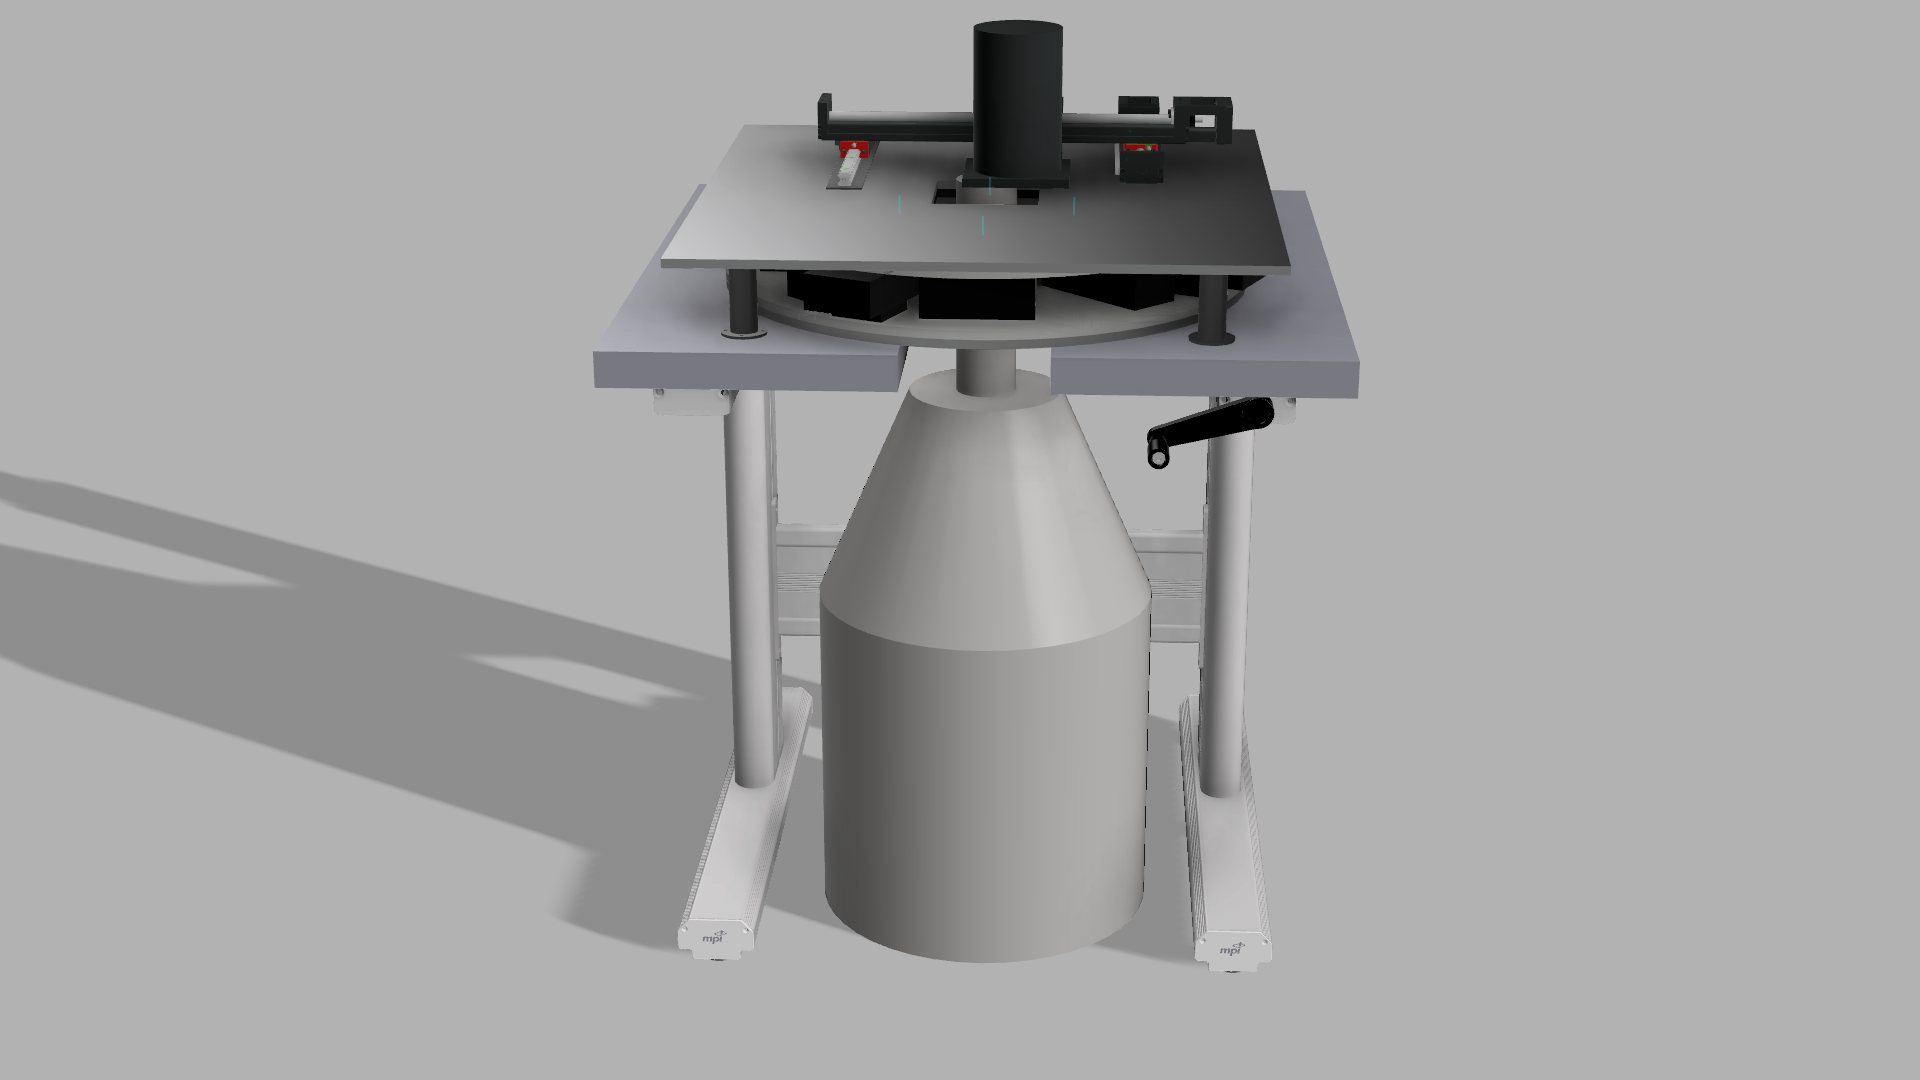
\includegraphics[scale=0.2]{final_setup.png}
\caption{3D view of the final scanning station. From top to bottom are shown the x-y scanning system with the collimator (black cylinder), the LYCCA ring (coïncidence setup) between the top table and the adjustable table and finally the dewar holding the crystal in its upper part (white cylinder).}
\label{3D_total}
\end{figure}

\subsection{Coïncidence setup} \label{coin_setup}

The coïncidence setup is made of a ring containing 12 LYCCA module \cite{LYCCA} surrounding the crystal to determine the height where the interaction took place in it. Horizontal absorbers made of tungsten are placed between the crystal and the modules to enable only some coïncidences to be detected in the zones between two absorbers (see Figure~\ref{coïncidence}). The crystal is placed in the middle of the ring and the collimated beam is directed from above towards the crystal.

\begin{figure}[!h]
\centering
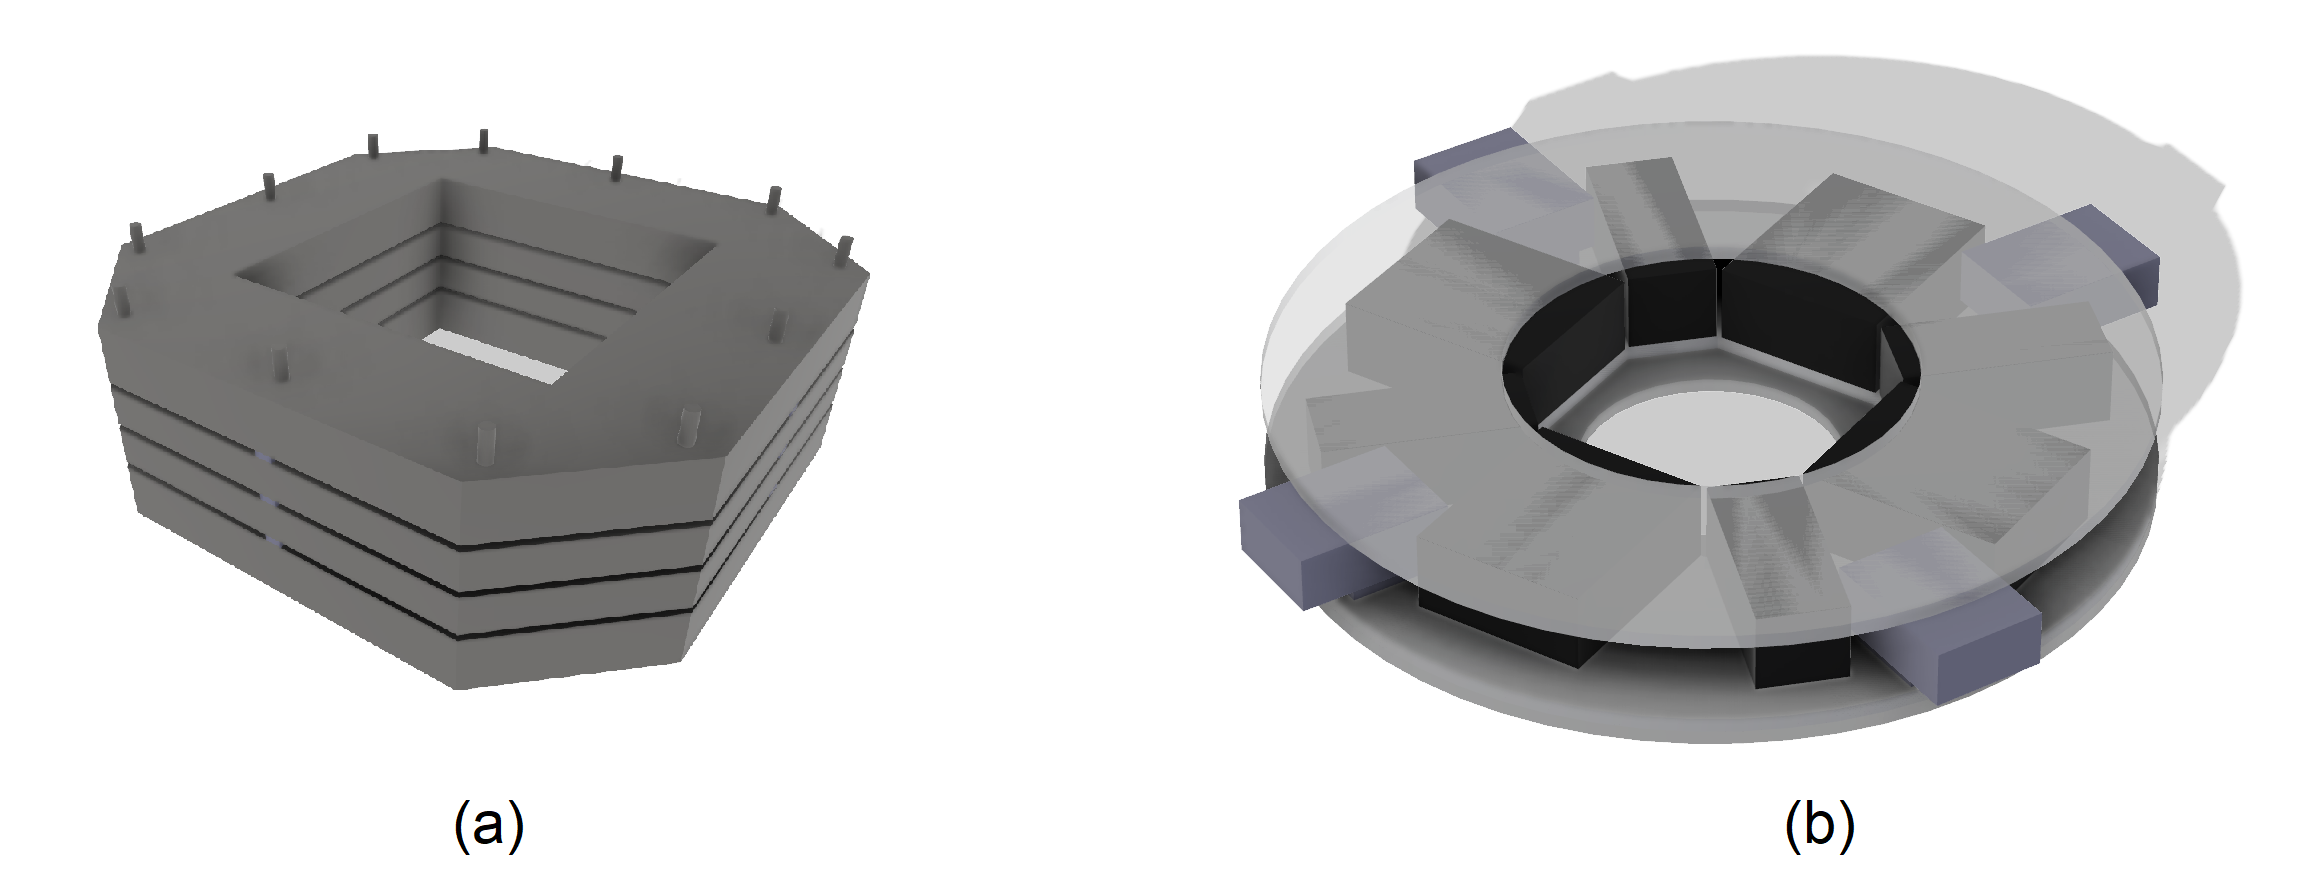
\includegraphics[scale=0.3]{coincidence.png}
\caption{3D views of the tungsten absorbers, (a), and the LYCCA ring, (b). On figure (a), each absorber is separated by little plastic pieces (in blue) to have a space where the coincident photons can be detected by the LYCCA modules. The LYCCA ring is made of twelve modules (black boxes) powered by four preamplifiers (blue boxes). The absorbers are mounted in the middle of the ring and the beam is directed towards the squared hole.}
\label{coïncidence}
\end{figure}

This part of the setup was the only part already built up that did not need to be designed.

\subsection{The holding structure}

This part of the setup was rather complicated to develop while some major constraints have to be taken into account. The first constraint is that the dewar must fit under the table while the crystal must be protruding above its plate to allow the coïncidence setup to be mounted on the table. The solution here was to design a table with a hole in the middle allowing this as can be seen on the final design of the table, Figure~\ref{table}. Another constraint was to have a height adjustable table. Indeed, the coïncidence setup could not cover the whole crystal to be scanned in height, having a height adjustable support for it could make a scan on the whole vertical direction of the crystal possible.

Finally, the loading capacity of the table should be sufficiently high while some pieces such as the absorbers (\ref{coin_setup}) or the collimator are made of tungsten for a global weight of around 60 to 70 kilograms, without counting other pieces, the total weight being estimated around 100 kilogramms. A 3D view of the table is shown on Figure~\ref{table}. On this first layer, the LYCCA ring will be mounted in the middle to match with the end of the cap coming from the dewar.

\begin{figure}[!h]
\centering
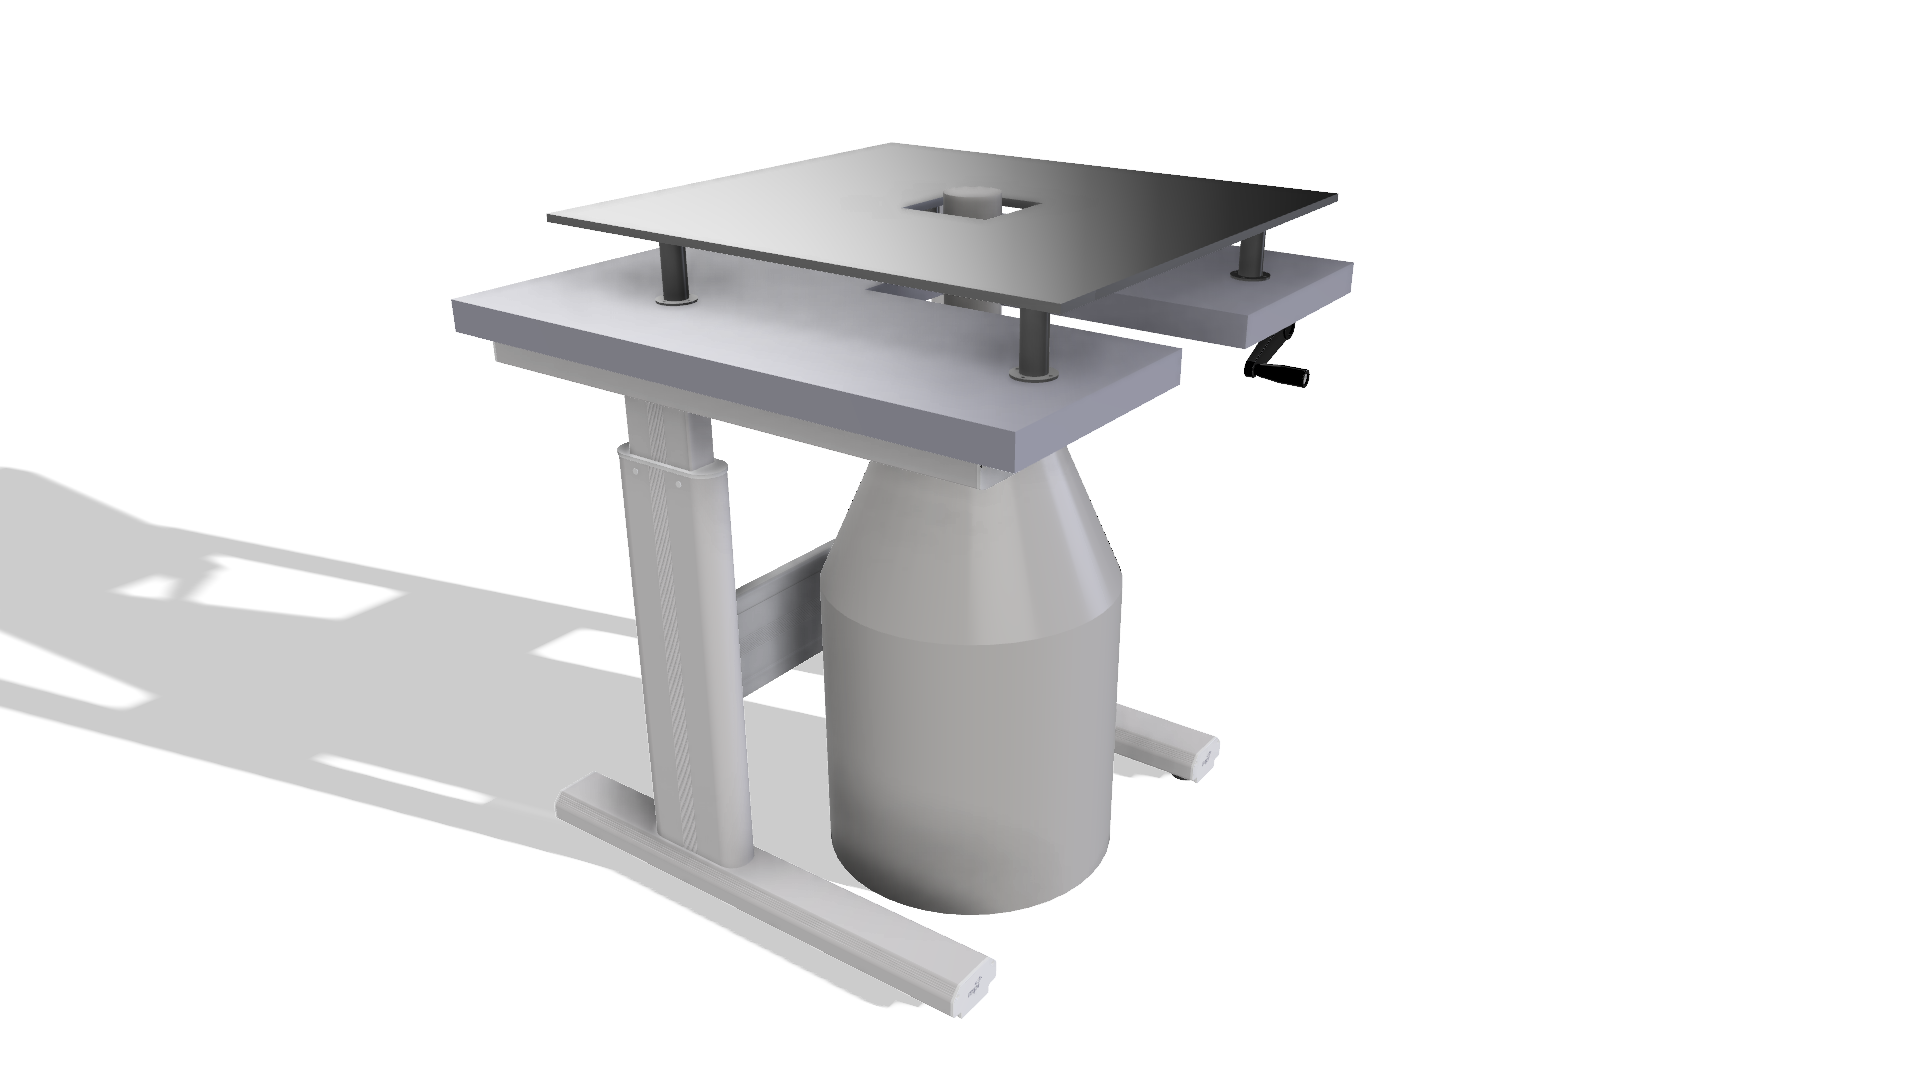
\includegraphics[scale=0.5]{table.png}
\caption{3D view of the table and the top plate. The dewar and the cryostat containing the crystal are also represented as they should go in the final setup. The coïncidence setup (absorbers and LYCCA ring, \ref{coin_setup}) fits between the table and the top plate to collect $90~\deg$ scattered photons from the crystal. The x-y scanning system (\ref{x-y}) is fixed on top of the plate.}
\label{table}
\end{figure}

The next step was thus to find a solution in order to put the x-y scanning system on top of the table. Again, this second layer should be quite resistant while a load of around 30 kilograms would then be added on top of it. In order for the directed beam to reach the crystal, a hole should be drilled in the middle of the top plate, matching the dimensions of the crystal to scan. As the bottom table is already height adjustable, this second layer did not need to be as well, reducing the constraints. For all these reasons, a thick plate of iron with a square hole in the middle was designed to be mounted on four legs fixed on the table in the four corners. The result presenting the structure of the setup is shown on figure~\ref{table}.

\subsection{The x-y scanning system} \label{x-y}

After the global structure of the scanning station was decided, certainly the most critical step was to develop the x-y scanning system. Indeed, this construction had to fulfill several conditions such as a rather good uncertainty on the positionning, the possibility to remote control the movement, a quite high load capacity, etc. After a few research and calls to different companies, the best option seemed to use two linear units and a linear guide and hang the collimator containing the source on one of them (see Figure~\ref{scan}). Linear units are devices that contain a rail and a wagon and use a screw going through the wagon to move it with a motor. Thus, a linear unit can move its wagon in one given direction. Thus, fixing two of those units on one another and perpendicular to each other should allow an object fixed on top to move in two different directions. The linear guide, which has basically the same role as the linear units except it is not motorized and then just follows the lead, is placed parallel to the first linear unit so that the one on top can be fixed to both, increasing the stability and load capacity of the construction.

The whole scanning system needs to be mounted on top of the principal structure so that the radioactive beam can be directed towards the crystal. As the linear units and the linear guide have holes, matching holes were drilled in the top plate at the correct positions in order to be able to cover the square hole in the middle of the plate. The last concerns about the units were to obtain a correct precision in their movement and to be sure that they could hold the collimator. The precision is only limited by the motors used to move the wagons, while the inner precision of the units is of the order to some microns, way better than what is needed here, as $0.1~mm$ seems reasonable. Thus the motors were chosen to match this requirement and to be powerful enough to push the wagon with the collimator (around $26~kg$). For the load, the linear units are not supposed to hold a great vertical load, but they can support a high torque in any direction. An arm protruding from the top unit was then designed to hold the collimator. This would minimise the vertical load applied on the wagon and maximise the torque, making this solution viable.

\begin{figure}[!h]
\centering
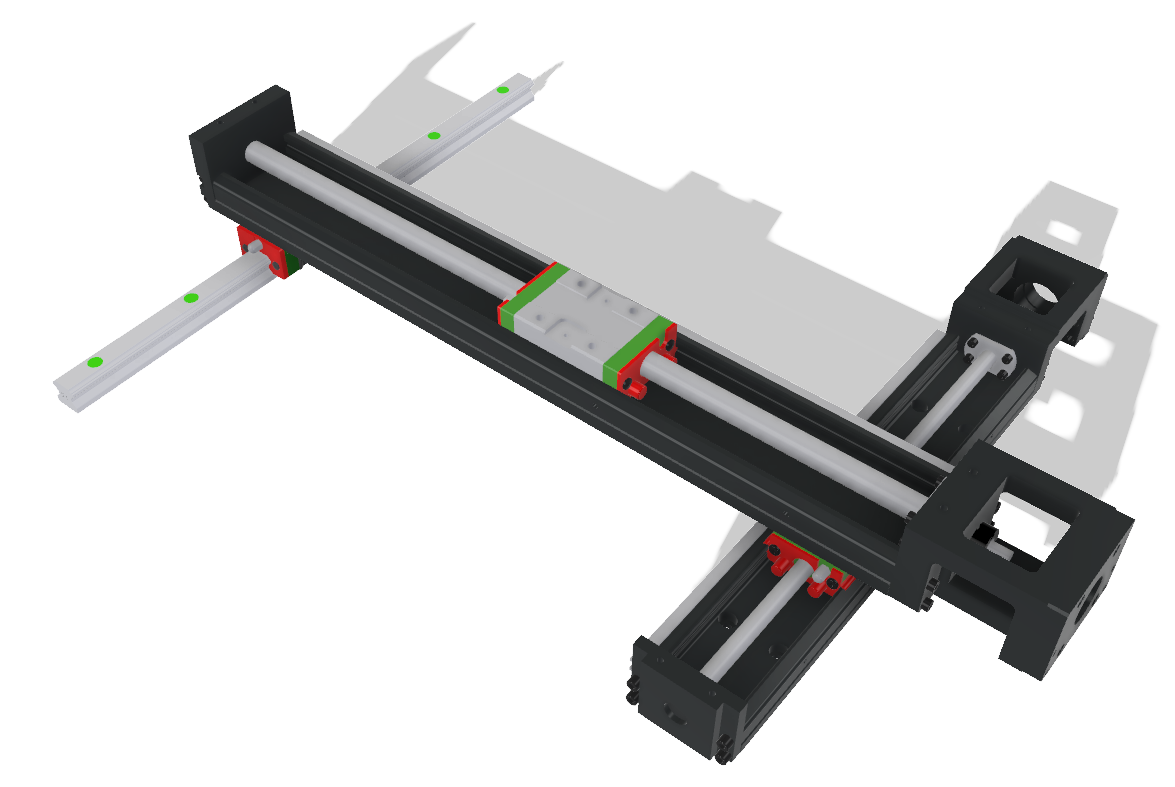
\includegraphics[scale=0.4]{position.png}
\caption{3D view of the x-y scanning system. The linear guide (grey) and linear unit (black) under are fixed on the top plate and allow a movement in one direction. The collimator arm with the collimator are fixed on the wagon of the linear unit on top which allows movement in the other direction.}
\label{scan}
\end{figure}

\begin{figure}[!h]
\centering
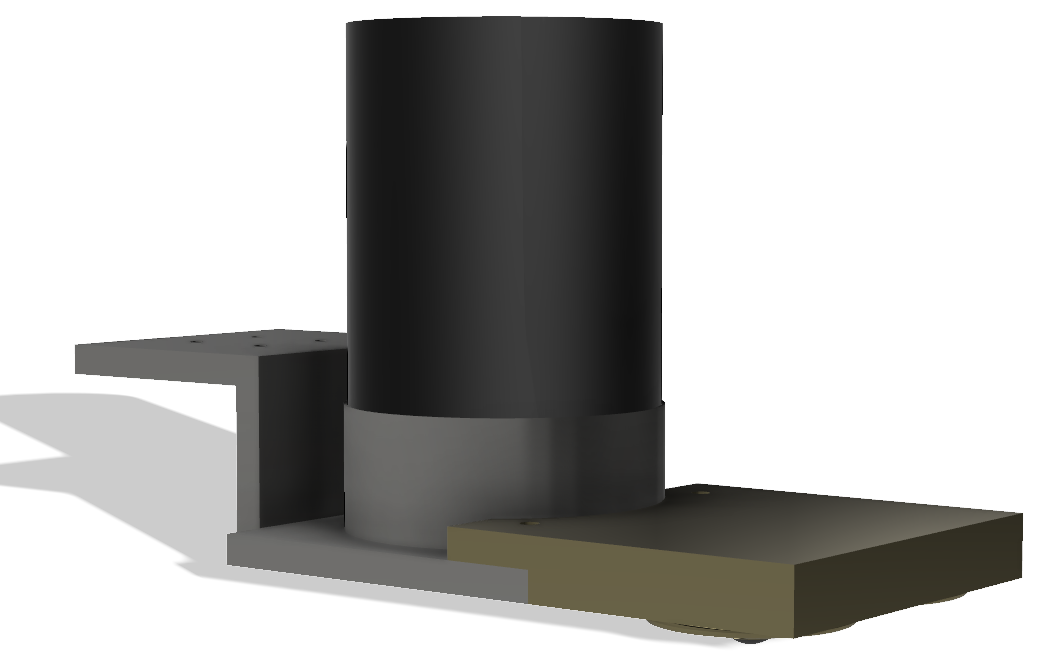
\includegraphics[scale=0.4]{Arm.png}
\caption{3D view of the arm holding the collimator (black). This 3D drawing shows the arm as it was first designed (grey part) and with an extension (golden part) that could be added in case the linear unit could not bear the collimator (this part was finally not needed).}
\label{arm}
\end{figure}

The collimator arm was the last piece of the setup to be designed and its ideal shape was quite hard to determine. The first thought was to build it as a stair, with the upper step being fixed on the wagon and the lower one holding the collimator. As the collimator is quite imposant and extremely dense (tungsten alloy to collimate the beam in a $1~mm$ hole going through it), a back up plan was designed using two spherical wheels on an extension of the arm that would allow the collimator to rest on the top plate, reparting the load on it (see Figure~\ref{arm}). To study the need for this extension, stress simulations were performed for two principal materials, aluminum and steel. The results, estimated for a load of $30~kg$ applied on the whole lower step, showed a maximum vertical deformationof around $0.3~mm$ for aluminum and $0.1~mm$ for steel. Such a deformation would lead to an uncertainty on the position of the beam on the crystal of $0.1~mm$ and $0.05~mm$ using aluminum and steel respectively. The solution that was kept was thus a steel arm, as shown on Figure~\ref{arm} and the back up plan with the extension was still kept in mind if the first tests with the regular arm were not satisfying.

\newpage

\section{Scanning the prototype detector}

While the scanning station was not already built and the different pieces took several months to arrive in Lund, measurements were performed with another setup that used material available in Lund. This was made to verify the measurements of resolution given by the company building the prototypes of detector, Canberra. These first measurements were also an opportunity to study the effect of capacitance of the detector and trapping on the resolution and compare both effects.

\subsection{Overall setup} \label{setup}

The setup uses three detectors: two scintillator detectors, placed on the sides (black squared boxes in Figure \ref{Setup}) and one semiconductor detector - hyperpure germanium detector - below the collimated source (grey cylinder in Figure \ref{Setup}). The source is placed on the top lead brick which contains a hole in the middle to collimate the radioactive source. In that position, the source is 97mm from the top of the crystal, which is 5mm from the top of the cryostat, and collimated in a 5mm hole through an 80mm lead brick. The source is covered by a little lead brick and the setup is shielded by lead to avoid propagation of gamma radiation away from the setup (see Figure \ref{Setup_front}).

\begin{figure}[!h]
\centering
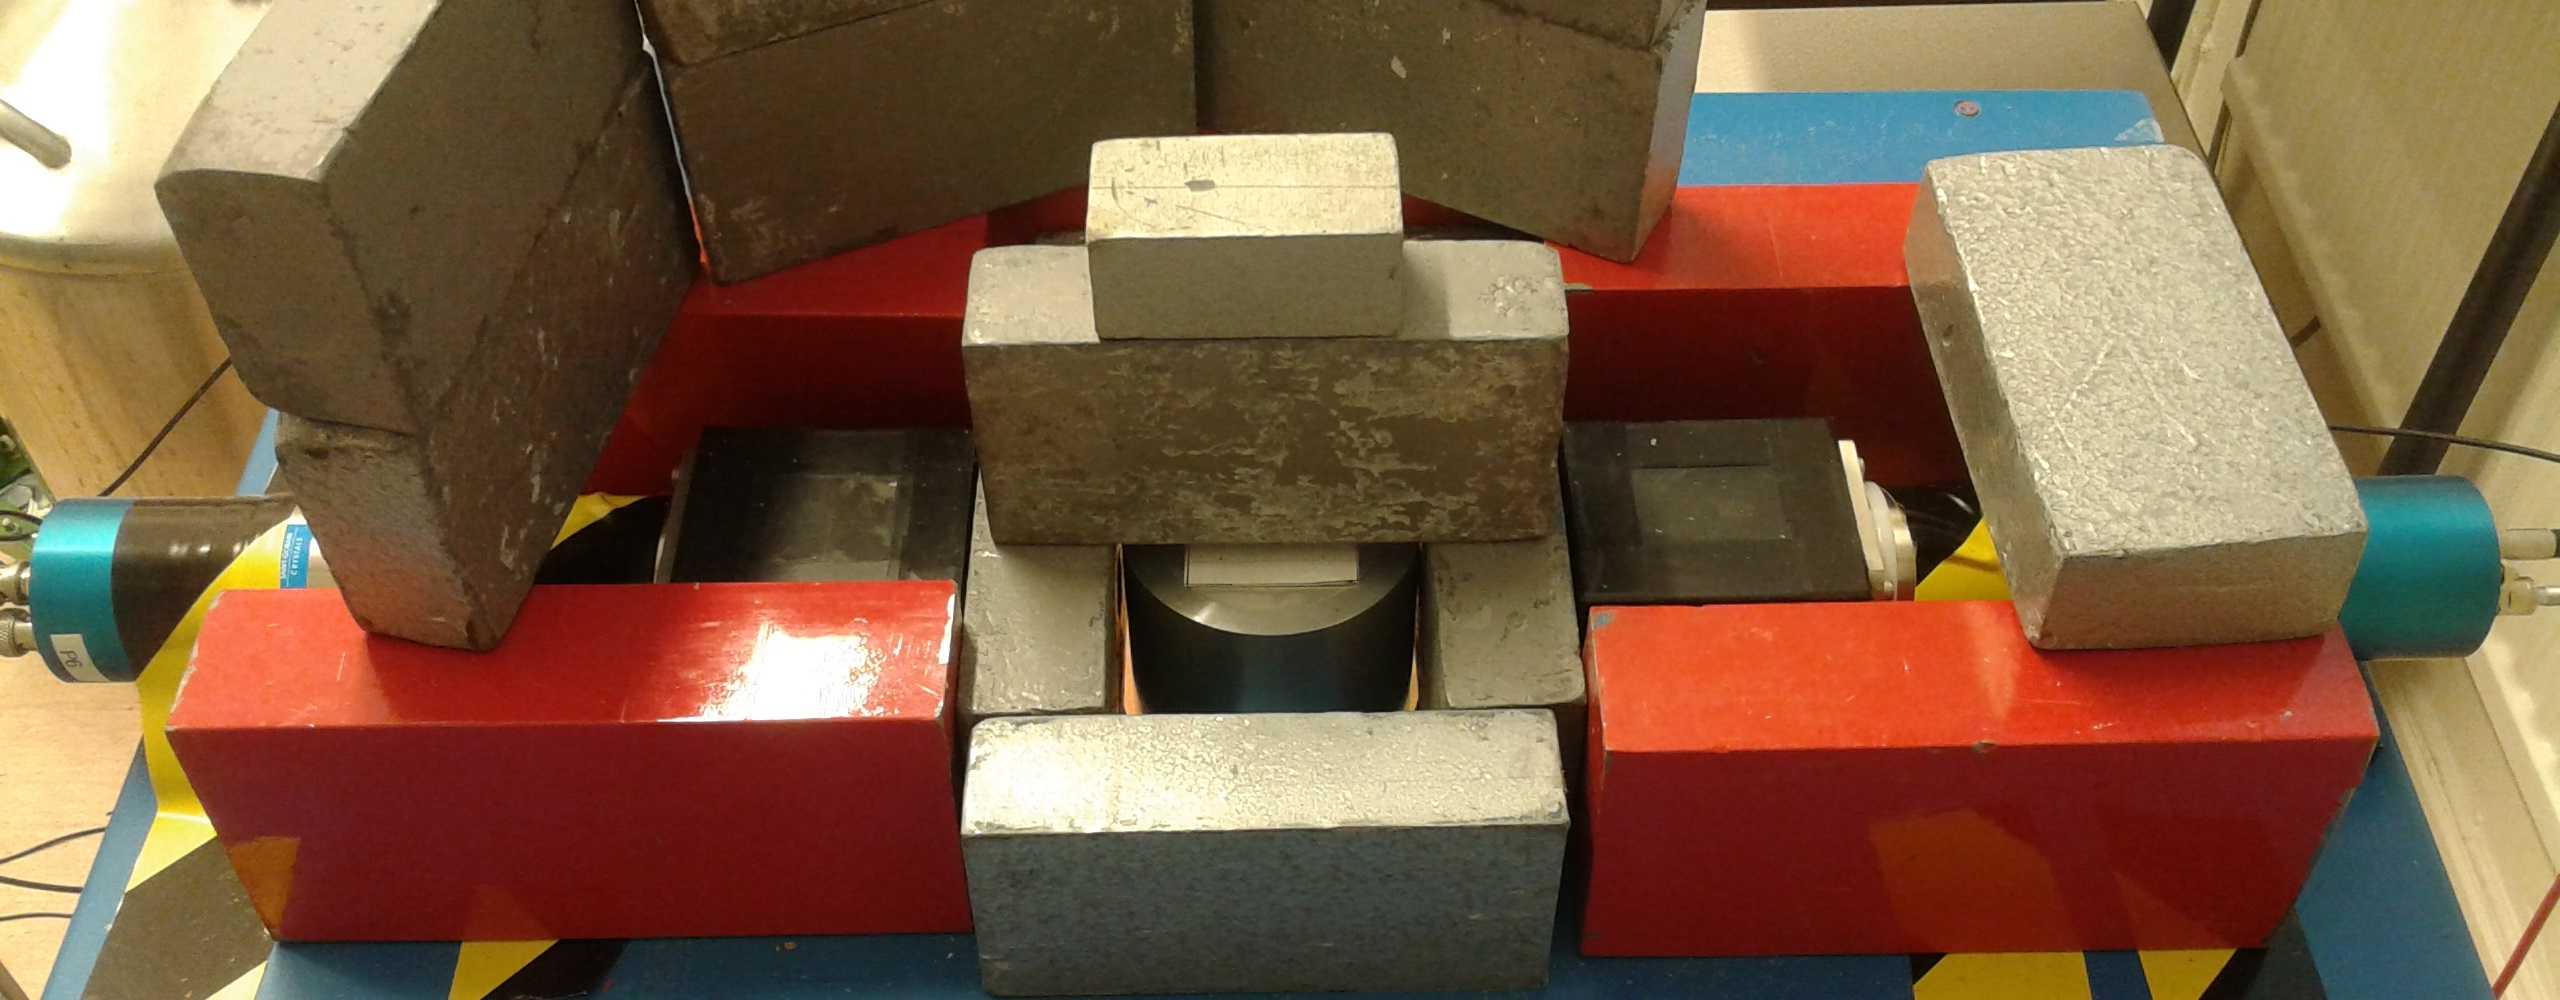
\includegraphics[scale=0.15]{New_setup_back.jpg}
\caption{Back of the original setup. The scintillator detectors are the black squared boxes on the sides of the germanium detector, placed in a cryostat (grey cylinder in the middle).}
\label{Setup}
\end{figure}

\begin{figure}[!h]
\centering
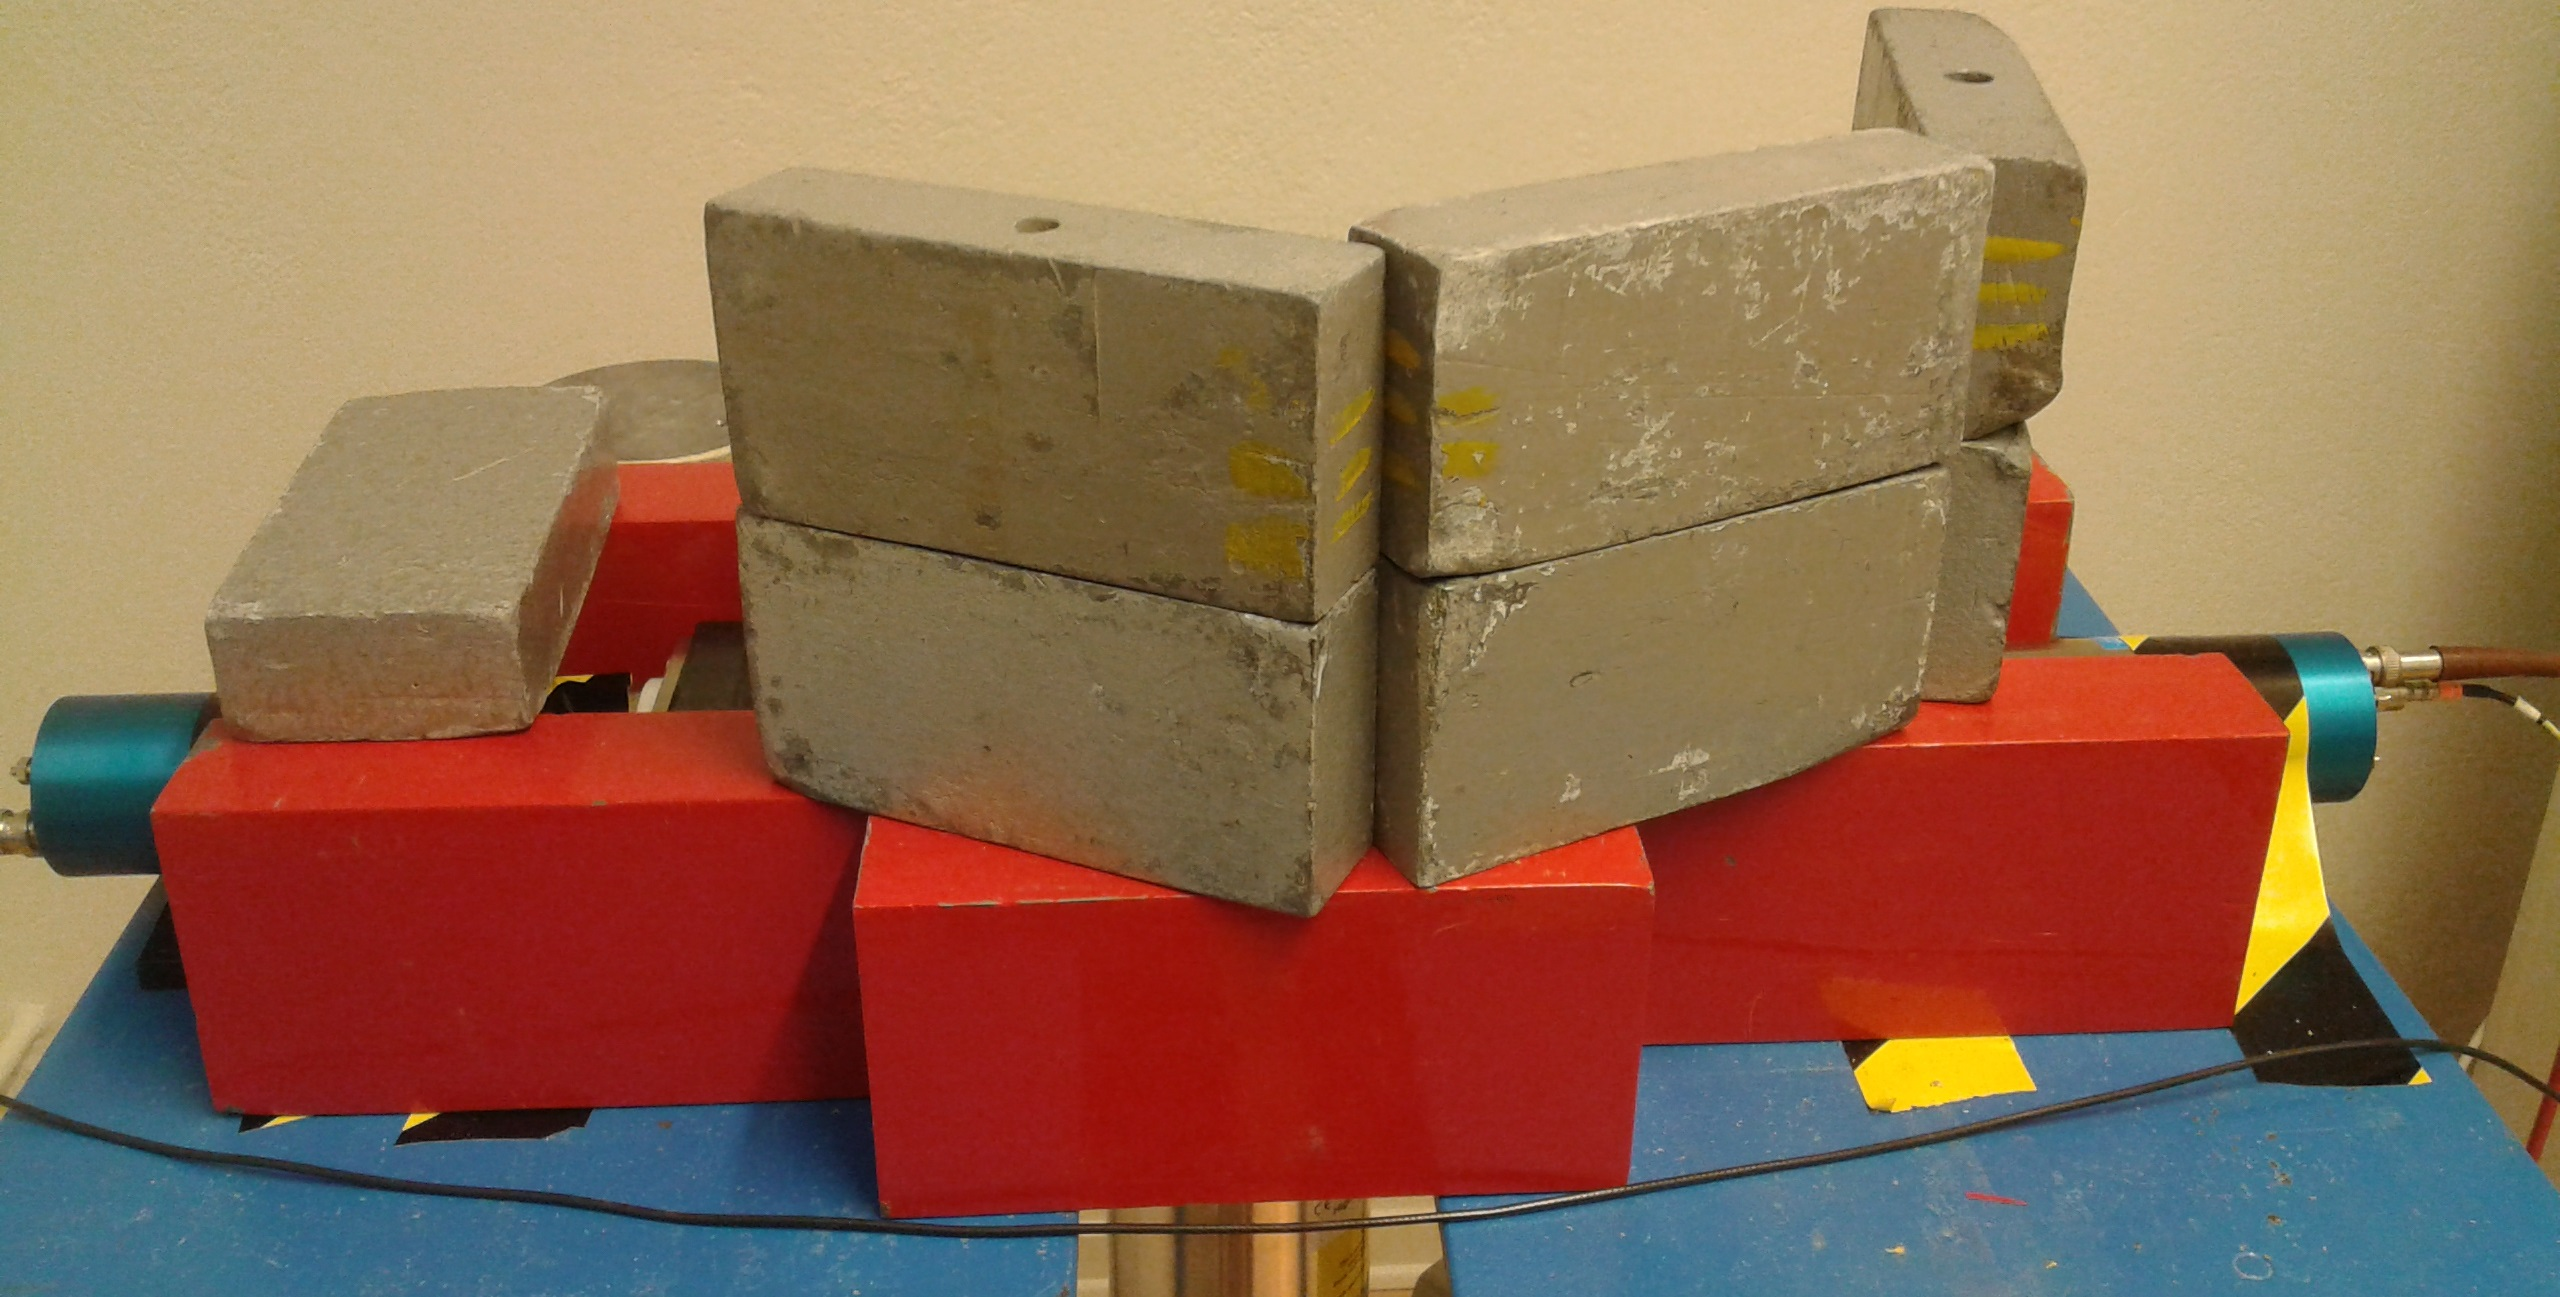
\includegraphics[scale=0.15]{New_setup_front.jpg}
\caption{Front side of the original setup (with the lead shielding). Two holed lead bricks can be seen on this picture as the one used to obtain a collimated beam.}
\label{Setup_front}
\end{figure}

\subsection{Process of measurement} \label{protocol}

For the first set of measurements, only the germanium detector was used but not the scintillator detectors. The goal of this experiment was to determine some spectral properties of the detector depending on the location of the collimated source such as the resolution of the crystal. Therefore, the source was directed onto five different points on the top of the crystal: one measurement was performed directing the beam in the center of the crystal surface, and four in the corners of the crystal surface. This was made possible by the use of a holed lead brick on top of which the source was positioned. The scanning was conducted as described below and two different cobalt sources were used, one of $^{60}$Co and one of $^{57}$Co.

In the case of $^{60}$Co, the source was held in one of the positions until the net area\footnote{In the analysis of the spectra, two areas need to be differenciated~: the total area, which gives the total number of counts between two channels, and the net area, which gives the number of counts between two channel substracted by the background.} of the studied peak (peak at $1332~keV$) contained at least 100~000 counts to match the measurement performed by the company manufacturing the detectors. Since the $^{57}$Co source was much less active, the measurement was stopped when the net area of the studied peak (peak at $122~keV$) contained around 1~000 counts.

The very first step was to perform the calibration. To do so, the two lines present in the spectrum of $^{60}$Co were used (lines at $1173~keV$ and $1332~keV$) and associated to a channel in the 8192 channel analyzer. In order to avoid a shift in the low energy range, the line at $122~keV$ in the spectrum of $^{57}$Co was also used. Then a linear fit was performed to get the the calibrated energies and then the equation of channels as a function of energy that was used in the analysis procedure later on (the data analysis is described in section~\ref{analysis}).

\subsection{Electronics}

For the first set of measurements, the scintillator detectors and the coincidence setup were not used, thus the electronics are relatively simple. The germanium detector is powered by a high voltage supply as explained in section~\ref{theory}. After going through a preamplifier, included in the cryostat, the signal is sent to an amplifier. Besides amplifying the signal, the amplifier also shapes it to a Gaussian. It is then digitized by an Analog to Digital Converter, ADC, and a multichannel analyzer sorts the digital values which are sent to the computer that collects the data using the Maestro software. Both the high voltage supply and the amplifier are Nuclear Instrumentation Modules (NIM, a standard set of modules) and are placed in a NIM crate that provides the necessary power for operation.

\subsection{Results and analysis} \label{analysis}

\subsubsection{First prototype}

The measurements that were conducted here had two main objectives. First, they were done in order to verify the values of the principal characteristics claimed by Canberra but this first experiment was also performed to get a first idea of how the crystals will be scanned with the final scanning system and what quantities to measure. This way, the detector was scanned following the protocol explained in section~\ref{protocol}.

The resolution of the detector, given by the full width at half maximum (FWHM), along with the shape of the peak, emphasized by the ratios between, the full width at tenth and fiftieth maximum, and the FWHM, were studied. The results are shown in the two tables below, both for the $^{60}$Co and $^{57}$Co source (Figure~\ref{recap}). For each source, the peaks in the spectra were fitted with Gaussians and the FWHM was deduced from the fit. As the fitting program uses the FWHM to optimise the fit, the value given by the Gaussian is the same as the real value that can be read from the data. This is not the case when it comes to the FWTM and FWFM and these values were directly read off the spectra without using the fit.

\begin{figure}[!h]
\centering
\caption{Recap charts of the obtained results using the $^{60}$Co and $^{57}$Co sources. $^{60}$Co and $^{57}$Co were used for calibration to avoid possible shifts in the low energy range.}
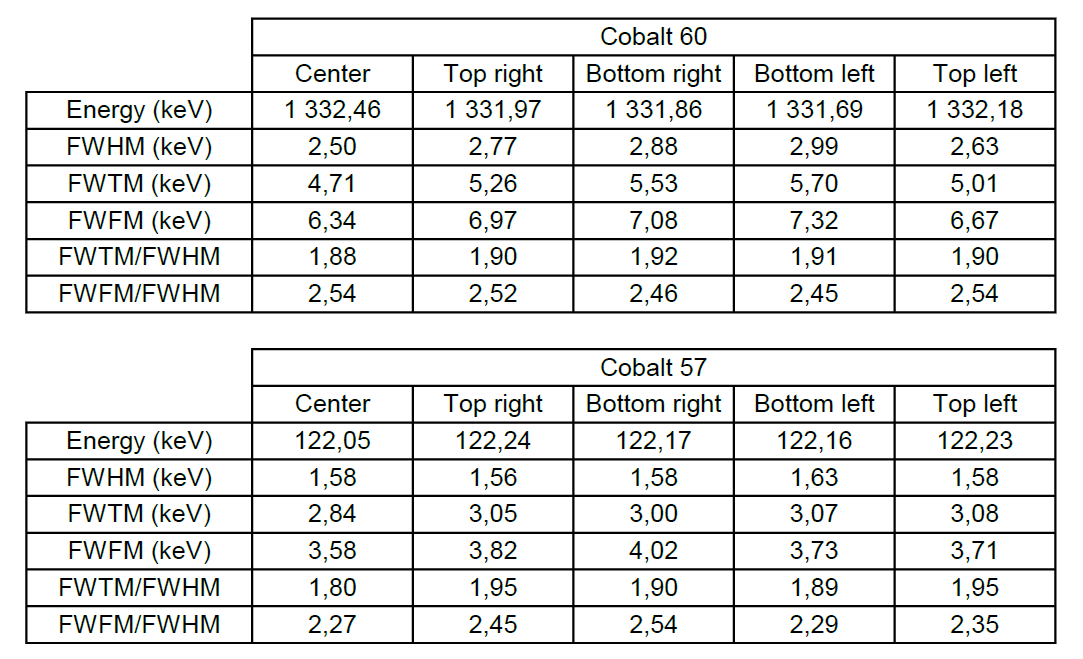
\includegraphics[scale=0.6]{Scan_Cos_2.png}
\label{recap}
\end{figure}

The very first thing we can notice in this set of measurments is that there is a shift in energy depending on where the beam was collimated. This shift in energy between the expected values (\cite{lit}) and the measured values goes up to around $0.8~keV$ if the beam is not directed towards the center of the crystal. It is normal that the measure of the peak energy in the center of the crystal is the closest to the energy we can find in the literature, while the calibration was made using this measurement and the measurement in the center with a $^{57}$Co source. This is also why the same measurement done in the center of the crystal with the $^{57}$Co source gives the closest result to the literature (STOPPED CORRECTIONS HERE) value. The shift in energy is more important in the range of high energies and thus for the results obtained with the $^{60}$Co source. This is not an observation that is really possible to explain, but the fact that the peaks are not seen at the same energy depending on where the beam is directed is still interesting to notice. As stated in different articles treating the subject, this could come from the difference of path the charge carriers need to travel depending if the interaction happens in a corner or in the center of the crystal. Indeed, as seen before in section~\ref{theory}, the more charge carriers have to travel to reach the electrodes and be collected, the more they are susceptible of being trapped in the crystal. This can imply a shift in energy and also differences in the measure of the resolution of the crystal as explained earlier.

The same observation can be done while looking at the resolution measured in the different parts of the crystal. As for the peak energy, the difference is not huge for measurements with the $^{57}$Co source. But for the second cobalt source, the resolution varies from $2.50~keV$ up to $2.99~keV$ which is quite a big difference. Nonetheless, these values of resolution are roughly in agreement with the values provided by Canberra for the $^{60}$Co, which were, for this first prototype, of $2.40~keV$ at $1332.5~keV$. The difference between both measurements in Lund and in Canberra can be explained by the different experimental conditions in which the measurements were done. The cryostat used with the crystal could influence the measured resolution, as welle as the electronics and the treatment protocol of the data. While the first is not critical, an improvement in the electronics used can change the values of the resolution by quite a lot and as the program used to analyse the data was not the same in both cases, this could also influence the measured FWHM. The real problem here is the huge difference between the resolution obtained at Lund and at Canberra for the $^{57}$Co source~: $1.59~keV$ were measured in Lund and $0.81~keV$ which means almost twice what the final goal is. This could be explained by the $^{57}$Co source used in Lund~: the source was too weak and the net area of 100~000 counts under the peak recommended by Canberra could not be reached. These values were measured with a net area of around 1~000 counts under the peak which was thus not pointing as high over the background as it should have.

Finally, the symmetry ratios have been calculated and compared to the values given by Canberra. Again, for the $^{57}$Co source, it may not make a lot of sense to look at those values, as the peak is not large enough to be analyzed in a proper way. The values obtained for the $^{60}$Co source are closer to the theoretical values than the values given by Canberra ($1.90$ and $2.50$ against $2.19$ and $ $), indicating that the peaks obtained on the spectra have a better Gaussian shape.

\subsubsection{Second prototype}

For the second prototype, the goal was just to do the measurements to check the values provided by Canberra for this prototype and the detector was not scanned as the first prototype. Instead, the source was just placed at the exact same distance from the cap as described in~\ref{setup} but not collimated using a lead brick, in order to get a proper number of counts per second. Results are shown in chart~\ref{recap2} for the different sources that were used.

\begin{figure}[!h]
\centering
\caption{Comparative chart of the obtained resolution using, from left to right, $^{241}$Am, $^{57}$Co, $^{60}$Co and $^{137}$Cs. $^{60}$Co and $^{57}$Co were used for calibration to avoid possible shifts in the low energy range.}
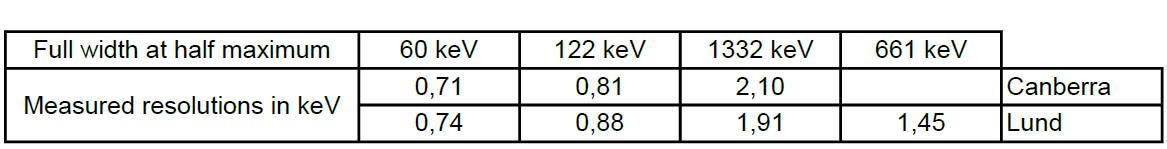
\includegraphics[scale=0.6]{result_2.png}
\label{recap2}
\end{figure}
Here the main focus was the measure of the resolution that should match the values given by Canberra (except for the cesium source, which was just performed to have a value of resolution in that range of energies). In the three cases that were given by Canberra, the results were in agreement and there was no critical measures like it was the case with the first crystal. The low energy resolution was found to be way higher than the one from the first crystal and overall the resolution increased quite significantly compared to the other detector. As for the first tested prototype, all these results are to be optimised using better electronics and cryostat as well as optimising the data analysis routine.

The shape factors of the peaks were also determined and matched quite well the ones given by the company, again slightly better than the ones from the first crystal (Figure~\ref{shape2}). The difference between these values can also be explained by the use of different electronics, that could lead to a better peak shape even if the differences are not significantly high.

\begin{figure}[!h]
\centering
\caption{Comparative chart of the peak shape at $1332.5~keV$ from the $^{60}$Co spectrum.}
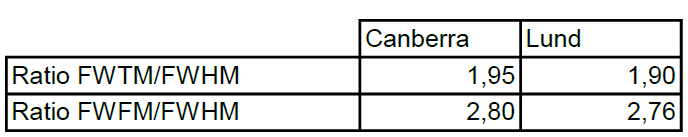
\includegraphics[scale=0.7]{shape.png}
\label{shape2}
\end{figure}
These results are quite interesting to analyse because the main difference between both crystals is the length of the hole in the middle, which is longer for the second prototype. What is important here is that the capacitance of the crystal increases with the length of the hole and thus, the resolution should decrease as the hole gets longer (see section~\ref{theory}). This is nonetheless not the case and the behaviour looks exactly the opposite, while the resolution increased with the second crystal. One of the reasons for that could be that as the length of the hole is increasing, the mean path of the charge carriers to travel to the inner electrode is decreasing and thus trapping is getting less important. As discussed earlier, effects of trapping can be really important on both the count rate and the resolution of the detector. From these results it could even be said that effects of trapping are much more important than capacitance as resolution was better for the second prototype. Trapping is also a big problem when it comes to the shape of the peak, which again confirms the fact that trapping was affected by the length of the hole and that a longer hole is better to obtain a good resolution in a semi-conductor detector. Finally, the quality of the crystal, which is not provided by the company, could highly affect the resolution of the detector and the first crystal may have been worse than the second one, also explaining the differences in resolution obtained.

\section{Conclusions}



\newpage

\bibliography{biblio}
\bibliographystyle{unsrt}

\end{document}